\documentclass[conference,10pt]{IEEEtran}

\usepackage{booktabs}
\usepackage{graphicx}
\usepackage{amsmath}
\usepackage{amssymb}
\usepackage{url}
\usepackage{microtype}
\usepackage{cite}

\newcommand{\Astar}{A$^\ast$}
\newcommand{\Dijkstra}{Dijkstra}
\newcommand{\code}[1]{\texttt{#1}}

\begin{document}

\title{When Does \Astar{} Save Work?\\ Controlled Experiments on Grids and Road Networks}

\author{
\IEEEauthorblockN{Elnur Haqqverdiyev and Rajab Iskandarli}
\IEEEauthorblockA{Department of Data Science and Artificial Intelligence\\
UFAZ, Advanced Data Structures and Algorithms, Fall 2026}
}

\maketitle

\begin{abstract}
\Astar{} is often described as Dijkstra's algorithm with a heuristic, but the
heuristic is not free: every generated vertex needs an estimate, and the heap
entry becomes larger.  We ask when the reduction in expanded vertices is large
enough to pay for this extra work.  We implement Dijkstra and \Astar{} in C++20
with the same CSR graph, binary heap, lazy deletion and search loop, and compare
them on five unit-cost grid families (open, random obstacles, clustered
obstacles, rooms and perfect maze) and on the SNAP California road network with
an ALT landmark heuristic.  The protocol is paired, pre-registered and frozen:
330 query instances, 3,600 timed runs, independent BFS distance oracles, and
median/IQR plus bootstrap and Wilcoxon analysis.  \Astar{} is dramatically
better on open grids (105.7x median time, 222.4x fewer expansions), clearly
better with random, clustered or room obstacles (12.8x, 12.8x and 8.7x time),
but \emph{slower} in mazes (0.81x, i.e. 24\% slower) because Manhattan distance
does not see the forced turns.  On the road graph, ALT with 8 landmarks gives
7.62x speedup and 11.54x fewer expansions; 16 landmarks improve further to
13.52x and 22.41x.  Time savings are systematically smaller than expansion
savings because \Astar{} costs about 1.2--2.0x more per settled vertex.  No
distance mismatch or timeout occurred.  The result is a practical rule rather
than a universal claim: \Astar{} pays when the heuristic is informative about
the actual remaining path.
\end{abstract}

\begin{IEEEkeywords}
shortest paths, \Astar{}, Dijkstra, binary heap, admissible heuristic, ALT,
road networks, experimental algorithmics, reproducibility.
\end{IEEEkeywords}

\section{Introduction}
Shortest-path queries are a basic primitive in routing,
network analysis and AI search.  Dijkstra's algorithm \cite{dijkstra1959} is the
standard exact method for non-negative edge weights; \Astar{} \cite{hart1968}
uses an estimate of the remaining distance to focus the search.  The textbook
intuition is that \Astar{} expands fewer vertices and is therefore faster.  In
practice, the estimate is evaluated at every generated vertex, its values enter
the heap key, and a weak heuristic can leave the explored region almost
unchanged.  The benefit is therefore conditional on both graph structure and
heuristic quality.

This paper asks the T01 question: \emph{how do graph structure and heuristic
strength change the number of expanded vertices and the runtime of \Astar{}
compared with Dijkstra, on unit-cost grids with obstacles and on a real-life
graph?}  We answer with a controlled experiment rather than a single benchmark.
The main contributions are:
\begin{itemize}
  \item a C++20 implementation with a documented CSR graph, binary heap,
        grid generators, Dijkstra, \Astar{}, Manhattan and ALT heuristics, and
        independent BFS/Floyd--Warshall oracles;
  \item a pre-registered protocol that separates expansion savings from time
        savings and pairs every \Astar{} run with the same Dijkstra query;
  \item a structure--heuristic map of when \Astar{} wins, including a clear
        negative result in mazes and a positive result on a real road network;
  \item an accounting of the per-expansion overhead that explains why time
        savings are smaller than expansion savings.
\end{itemize}

Section~\ref{sec:background} reviews the algorithms.  Section~\ref{sec:data}
describes the graphs and Section~\ref{sec:method} the implementation and
protocol.  Section~\ref{sec:results} reports the measurements; Sections
\ref{sec:discussion} and \ref{sec:threats} discuss the meaning and limits.

\section{Background}
\label{sec:background}

\subsection{Dijkstra and \Astar{}}
Let $G=(V,E,w)$ be a graph with $w(u,v)>0$.  Dijkstra maintains a tentative
distance $g(v)$ and repeatedly settles the unsettled vertex with minimum $g$.
With a binary heap and lazy deletion the complexity is
$O((n+m)\log n)$ in the worst case, where $n=|V|$ and $m=|E|$.
\Astar{} additionally uses a heuristic $h(v)$ estimating the distance from $v$
to the target $t$, and orders the open list by
\begin{equation}
  f(v)=g(v)+h(v).
\end{equation}
If $h$ is admissible, $h(v)\le d(v,t)$, \Astar{} returns a shortest path; if it
is consistent, $h(u)\le w(u,v)+h(v)$, settled vertices never need reopening
\cite{hart1968,russell2020}.  Both heuristics used here are consistent.

\subsection{ALT landmarks}
For an undirected graph and exact distances $d(L,v)$ from a landmark $L$,
the triangle inequality gives
\begin{equation}
  |d(L,v)-d(L,t)| \le d(v,t).
\end{equation}
The ALT heuristic takes the maximum over a set $\mathcal{L}$ of landmarks
\cite{goldberg2005}:
\begin{equation}
  h(v)=\max_{L\in\mathcal{L}} |d(L,v)-d(L,t)|.
  \label{eq:alt}
\end{equation}
It is admissible because every term is a lower bound, and consistent because
each term changes by at most the edge weight across an edge.  The landmark
distance tables are computed by BFS before any timed search.

\subsection{Expansions versus time}
Let $X$ be the number of settled vertices.  If the average cost of an expansion
is $c_D$ for Dijkstra and $c_A$ for \Astar{}, then
\begin{equation}
  \frac{T_D}{T_A}=\frac{X_D\,c_D}{X_A\,c_A}.
\end{equation}
The expansion ratio $X_D/X_A$ overstates the time ratio whenever $c_A>c_D$.
This decomposition is the main explanatory tool of the paper.

\section{Data}
\label{sec:data}

\subsection{Grid controls}
Grids are square, row-major and 4-neighbour with unit edge cost.  A blocked cell
is an isolated vertex; only the largest 4-connected component is used for query
selection.  We use five families:
\begin{itemize}
  \item \textbf{open}: no blocked cells;
  \item \textbf{random}: independent blocking with probability 0.20;
  \item \textbf{clustered}: 30\% blocked in random circular blobs;
  \item \textbf{rooms}: walls every 16 cells with one door per room-boundary
        segment;
  \item \textbf{maze}: a perfect maze generated by iterative randomised DFS.
\end{itemize}
Sizes are $128^2$, $256^2$, $512^2$ and $1024^2$ cells.  These families isolate
different structural effects: exact geometric guidance (open), local detours
(random), long detours (clustered/rooms) and forced corridors (maze).

\subsection{Real road network}
We use SNAP \code{roadNet-CA}, the California road network
\cite{snap}.  The SNAP page reports 1,965,206 nodes and 2,766,607 edges.  We read
the 5,533,214 directed arcs, symmetrise each road segment, remove self-loops and
duplicates, take the largest connected component and compact the vertex ids.
The resulting graph has \textbf{1,957,027 vertices} and \textbf{2,760,388
undirected edges} (5,520,776 CSR arcs), average degree $\approx 2.82$.
SNAP does not provide road lengths or travel times, so we use \textbf{unit hop
cost} rather than inventing a weighted interpretation.  The result is therefore
a hop-count result; it is not a claim about travel-time routing.

\begin{table}[!t]
\centering
\caption{Experimental graphs and query budget.}
\label{tab:data}
\footnotesize
\setlength{\tabcolsep}{3pt}
\begin{tabular}{lrrrr}
\toprule
Data & graphs & queries & repeats & timed runs\\
\midrule
Grid controls & 20 & 300 & 3 & 2,700\\
Road network & 1 & 30 & 5 & 900\\
\midrule
Total & 21 & 330 & -- & 3,600\\
\bottomrule
\end{tabular}
\end{table}

\section{Implementation and Protocol}
\label{sec:method}

\subsection{Graph, heap and search}
The graph is stored in compressed sparse row (CSR) form: \code{offsets[n+1]},
\code{targets[m]} and \code{weights[m]} use $O(n+m)$ memory, degree is $O(1)$
and neighbour iteration is $O(\deg u)$.

The binary heap is an array-based min-heap with duplicate entries and lazy
deletion.  \code{push} and \code{pop} are $O(\log n)$ worst case; \code{top} is
$O(1)$.  There is no decrease-key: a popped entry is stale if its $g$ differs
from the current tentative distance or if the vertex is already closed.  Two
deterministic tie-breaks are compared:
\code{node\_id} uses $(f,\mathit{id})$; \code{larger\_g} uses $(f,-g,\mathit{id})$.

Both algorithms call the \emph{same} \code{shortest\_path} routine.  A null
heuristic is Dijkstra; a non-null heuristic is \Astar{}.  This guarantees the
same CSR traversal, heap, relaxation and stopping rule.  The search stops when
the target is popped and settled.  Timed runs do not reconstruct paths;
correctness runs do.  Scratch distance/closed/parent arrays are reused and reset
in $O(1)$ with a generation stamp, so allocation is outside the timed region.

\subsection{Heuristics}
On grids we use Manhattan distance
\begin{equation}
  h(v)=|\mathit{row}(v)-\mathit{row}(t)|+|\mathit{col}(v)-\mathit{col}(t)|.
\end{equation}
It is admissible and consistent for 4-neighbour unit grids, with or without
obstacles.

On the road graph we use ALT \eqref{eq:alt} with 16 landmarks selected by
deterministic farthest-point sampling.  The first landmark is a fixed seed;
each next landmark maximises the minimum BFS distance to the already selected
landmarks.  The main treatment uses $K=8$; $K=1,4,16$ are secondary treatments.

\subsection{Correctness first}
Before timing, the test suite checks: heap order against a reference priority
queue; a hand-computed weighted graph against Floyd--Warshall; a hand-checked
$5\times5$ wall grid with distance 8; a no-path grid; all five grid families
against independent BFS; ALT admissibility and consistency for every free
vertex; tie-break distance equivalence; and a sample of real-graph queries with
edge-by-edge path validation.

Every benchmark query is also checked against BFS before it is recorded.  A
distance mismatch aborts the run.  Timeouts are recorded as \code{timeout},
never silently dropped.  All 3,600 main runs returned \code{ok} and matched the
oracle; no timeout occurred.

\subsection{Queries and timing}
Queries are selected by BFS only, independently of Dijkstra/\Astar{}.  For a
random source, BFS gives eccentricity $d_{\max}$; targets are sampled in three
bands: short $[0.08,0.25]d_{\max}$, medium $[0.40,0.60]d_{\max}$ and long
$[0.80,0.97]d_{\max}$.  Each grid has 5 sources (15 queries); the road graph has
10 sources (30 queries).

Each treatment gets one untimed warm-up per graph.  Grid queries are repeated
three times and road queries five times; the median is the query-level summary
and the raw repeats are kept.  Dijkstra and \Astar{} run on the same query and
their order alternates.  The timed region contains only the search call;
graph construction, BFS query selection and landmark tables are outside it.
A 30 s per-search cap is checked every 4096 pops and a 4 GiB process cap is
applied externally.  Runs are pinned to one CPU with \code{taskset}.

\begin{table}[!t]
\centering
\caption{ADT interfaces and worst-case costs ($n$ vertices, $m$ arcs).}
\label{tab:adt}
\footnotesize
\setlength{\tabcolsep}{3pt}
\begin{tabular}{p{2.6cm}p{3.7cm}}
\toprule
Component & Interface and cost\\
\midrule
CSR graph & neighbour loop $O(\deg u)$; degree $O(1)$; memory $O(n+m)$\\
Binary heap & push/pop $O(\log n)$; top $O(1)$; lazy deletion\\
Search & Dijkstra $h\equiv0$; \Astar{} $f=g+h$; same loop\\
Manhattan & $O(1)$ per estimate; admissible/consistent\\
ALT & $O(K)$ per estimate; $K$ landmark tables\\
Oracle & BFS $O(n+m)$; Floyd--Warshall $O(n^3)$ for tiny tests\\
\bottomrule
\end{tabular}
\end{table}

\subsection{Counters and statistics}
\emph{Expanded} is a popped entry that is not stale and not already closed
(the target counts when popped).  \emph{Pushed} counts every heap insertion,
including the source and every successful decrease.  \emph{Stale\_popped}
counts popped entries whose $g$ is outdated or whose vertex is closed.
\emph{Relaxed\_edges} counts outgoing arcs inspected from expanded vertices.
\emph{Heuristic\_calls} counts heuristic estimates (zero for Dijkstra).

We report medians and interquartile ranges over query-level medians.  Confidence
intervals for medians use 10,000 paired bootstrap resamples.  Paired Wilcoxon
signed-rank tests are reported for time and expansions.  Within-query repeat
variation is reported as a coefficient of variation (CV); the median CV was
7.2\% for grid Dijkstra, 10.1\% for grid \Astar{}, 7.4\% for road Dijkstra and
9.6\% for road \Astar{} ($K=8$).  Expansions were identical across repeats.

\section{Results}
\label{sec:results}

\subsection{Grid families}
Table~\ref{tab:grid} gives the main treatment (Manhattan, \code{larger\_g}).
Ratios are Dijkstra/\Astar{}; values above 1 mean \Astar{} wins.  The open grid
is the best case: \Astar{} expands 222.4x fewer vertices and is 105.7x faster in
the median, and it is faster on 100\% of queries.  Random and clustered
obstacles still give a clear win (21.4x and 22.9x fewer expansions; 12.8x time),
but the advantage is an order of magnitude smaller than on the open grid.
Rooms are weaker still: 14.3x expansions and 8.7x time.

The maze is the counterexample.  The expansion ratio is 1.02 (about 2\% fewer
expansions for \Astar{}) and the time ratio is 0.81, so \Astar{} is about 24\%
\emph{slower}.  Manhattan distance sees the straight line to the target but not
the forced turns of the maze.  \Astar{} pays the heuristic cost without changing
the explored region.

\begin{table}[!t]
\centering
\caption{Grid results, Manhattan heuristic, \code{larger\_g} tie-break.  Ratio
is Dijkstra/\Astar{}; IQR in parentheses.}
\label{tab:grid}
\footnotesize
\setlength{\tabcolsep}{2.5pt}
\begin{tabular}{lcccc}
\toprule
Family & Time ratio & Expansion ratio & A* faster\\
\midrule
Open & 105.7 (54.9--249.3) & 222.4 (105.1--490.3) & 100\%\\
Random 20\% & 12.8 (7.2--21.9) & 21.4 (11.3--31.7) & 98\%\\
Clustered 30\% & 12.8 (7.0--34.6) & 22.9 (11.7--67.8) & 98\%\\
Rooms & 8.7 (5.6--17.0) & 14.3 (8.4--25.6) & 100\%\\
Maze & \textbf{0.81} (0.75--0.94) & \textbf{1.02} (1.00--1.05) & 17\%\\
\bottomrule
\end{tabular}
\end{table}

\begin{figure*}[!t]
  \centering
  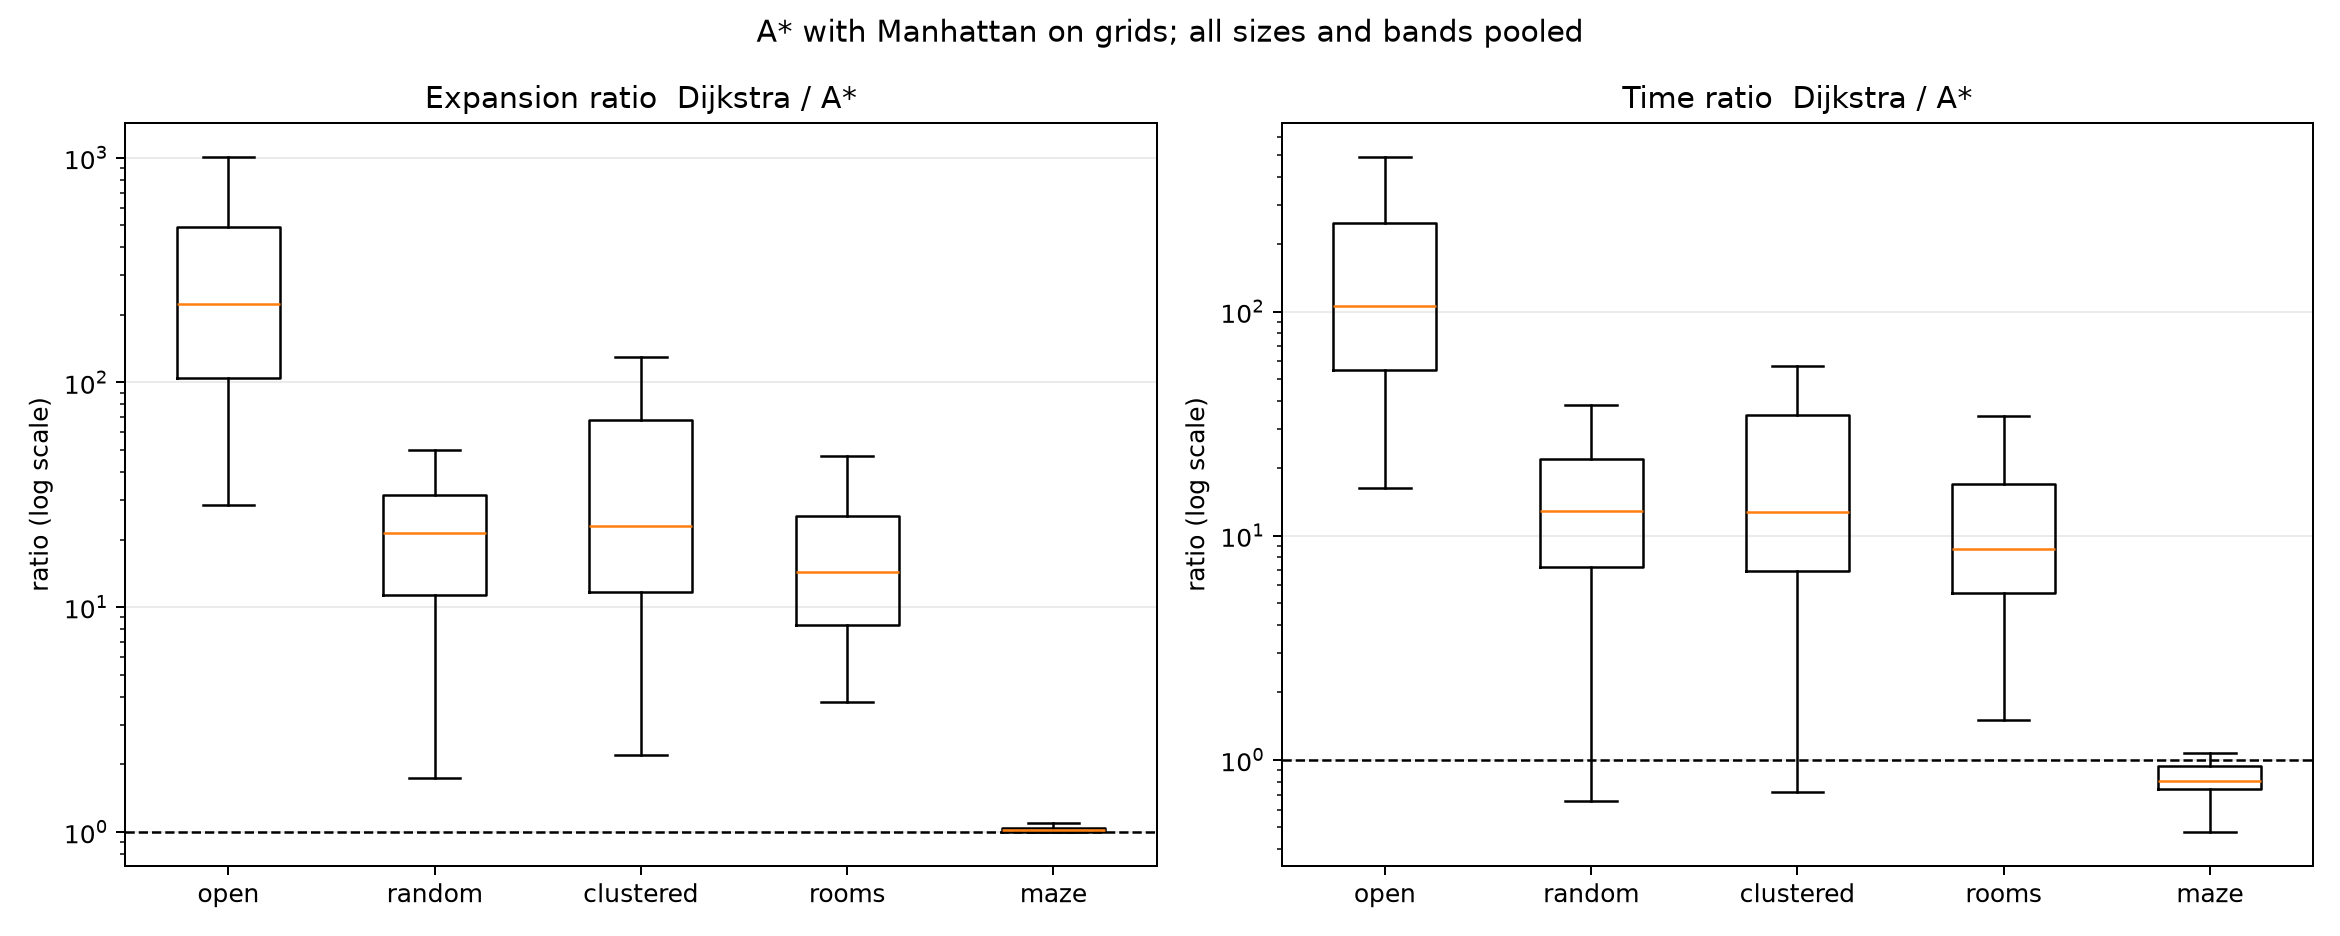
\includegraphics[width=0.78\textwidth]{../figures/grid_ratios_by_family.png}
  \caption{Expansion and time ratios for the five grid families, all sizes and
  distance bands pooled.  The horizontal line is parity.  The maze is below
  parity in time even though its expansion ratio is near one.}
  \label{fig:grid}
\end{figure*}

The open-grid advantage grows with size: at $128^2$ the median is 45.5x time
and 94.4x expansions; at $1024^2$ it is 389.9x and 696.3x.  Random grids are
roughly flat in ratio (12.0x at $128^2$, 21.0x at $1024^2$), while rooms do not
improve monotonically (7.6x, 8.7x, 11.4x, 8.7x).  The maze ratio rises from
0.75x to 0.97x as the fixed overhead becomes small relative to the search, but
\Astar{} never becomes faster in the median.

Distance bands are not a universal explanation.  On the open grid, long queries
benefit more than short ones (156.0x vs 83.5x time).  On random grids the
opposite ordering appears (long 11.5x vs short 14.4x): a long random query has
more opportunity to accumulate detours that Manhattan cannot predict.
Structure, not distance alone, controls the benefit.

\subsection{Real road network}
Table~\ref{tab:real} reports ALT.  With one landmark the expansion saving is
real (1.96x) but the time saving is not statistically significant (1.29x,
$p=0.13$): the heuristic is too weak to pay for itself.  With 4, 8 and 16
landmarks both differences are significant ($p<10^{-8}$).  The main treatment,
$K=8$, is 7.62x faster and expands 11.54x fewer vertices; $K=16$ reaches 13.52x
and 22.41x.

The K=16 result rejects the expectation of a plateau at K=8: paired on the same
30 queries, K=16 uses about 21\% less time and 25\% fewer expansions than K=8
($p<10^{-4}$).  More landmarks keep tightening the bound faster than their
per-expansion cost grows on this road graph.

\begin{table}[!t]
\centering
\caption{Road network results with ALT; ratio is Dijkstra/\Astar{}.}
\label{tab:real}
\footnotesize
\setlength{\tabcolsep}{3pt}
\begin{tabular}{lcccc}
\toprule
Treatment & Time ratio & Expansion ratio & Time saving & Faster\\
\midrule
K=1 & 1.29 (0.93--1.75) & 1.96 (1.44--2.44) & 22.5\% & 70\%\\
K=4 & 4.75 (2.38--7.71) & 7.26 (3.76--10.86) & 78.9\% & 100\%\\
K=8 & \textbf{7.62 (4.38--16.65)} & \textbf{11.54 (7.06--25.66)} & 86.8\% & 100\%\\
K=16 & \textbf{13.52 (7.64--25.25)} & \textbf{22.41 (12.94--38.70)} & 92.6\% & 100\%\\
\bottomrule
\end{tabular}
\end{table}

\begin{figure*}[!t]
  \centering
  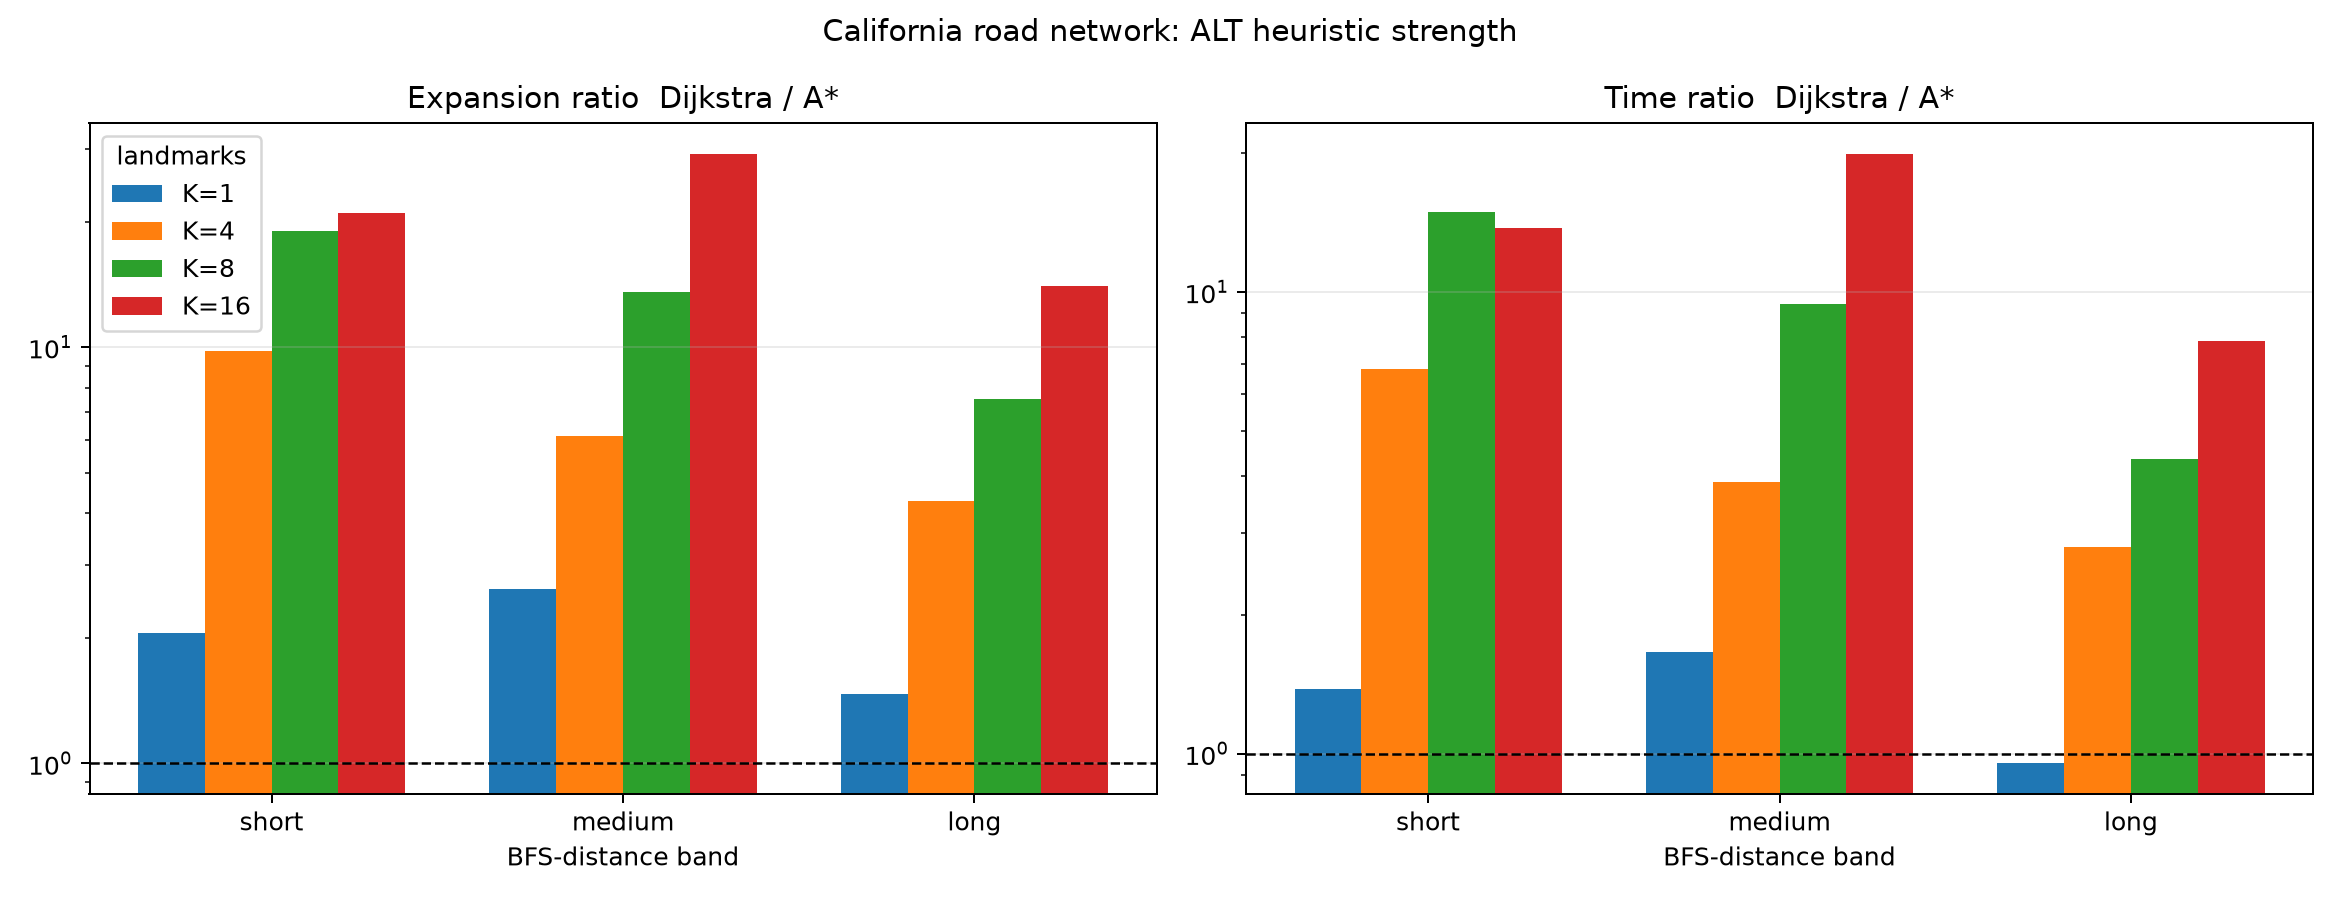
\includegraphics[width=0.78\textwidth]{../figures/real_ratios_by_band_k.png}
  \caption{Road network: expansion and time ratios by BFS-distance band and
  number of ALT landmarks.  The y-axis is logarithmic; the dashed line is
  parity.  The K=1 time ratio on long queries is below one.}
  \label{fig:real}
\end{figure*}

By band (K=8), the time ratios are 14.9x (short), 9.4x (medium) and 4.3x
(long); expansion ratios are 19.1x, 13.5x and 7.5x.  Absolute work still grows
with distance: median long-query \Astar{} expands 247,065 vertices and takes
99 ms, versus 448 ms for Dijkstra.  A long road route gives the landmark bound
more chances to be loose, so the ratio is smaller even though the absolute
saving is large.

\subsection{Why time differs from expansions}
Table~\ref{tab:cost} shows the measured cost per expanded vertex.  \Astar{}
costs 1.2--2.0x more per expansion.  On the open grid the expansion ratio is
222.4x but the time ratio is only 105.7x; on random grids 21.4x becomes 12.8x.
In the maze the cost ratio is 1.21x and the expansion ratio is 1.02x, so the
time ratio is 0.81x: the extra work has no compensating reduction in
expansions.  On the road graph, Dijkstra costs 234.5 ns per expansion, ALT K=8
372.9 ns (1.59x) and K=16 393.7 ns (1.68x).

\begin{table}[!t]
\centering
\caption{Cost per expanded vertex (ns), medians.}
\label{tab:cost}
\footnotesize
\setlength{\tabcolsep}{3pt}
\begin{tabular}{lccc}
\toprule
Data & Dijkstra & A* & Ratio\\
\midrule
Open grid & 142.2 & 288.3 & 2.03x\\
Random grid & 156.5 & 254.1 & 1.62x\\
Clustered grid & 126.7 & 245.0 & 1.93x\\
Rooms grid & 146.0 & 270.4 & 1.85x\\
Maze & 64.9 & 78.8 & 1.21x\\
Road, ALT K=8 & 234.5 & 372.9 & 1.59x\\
\bottomrule
\end{tabular}
\end{table}

\begin{figure}[!t]
  \centering
  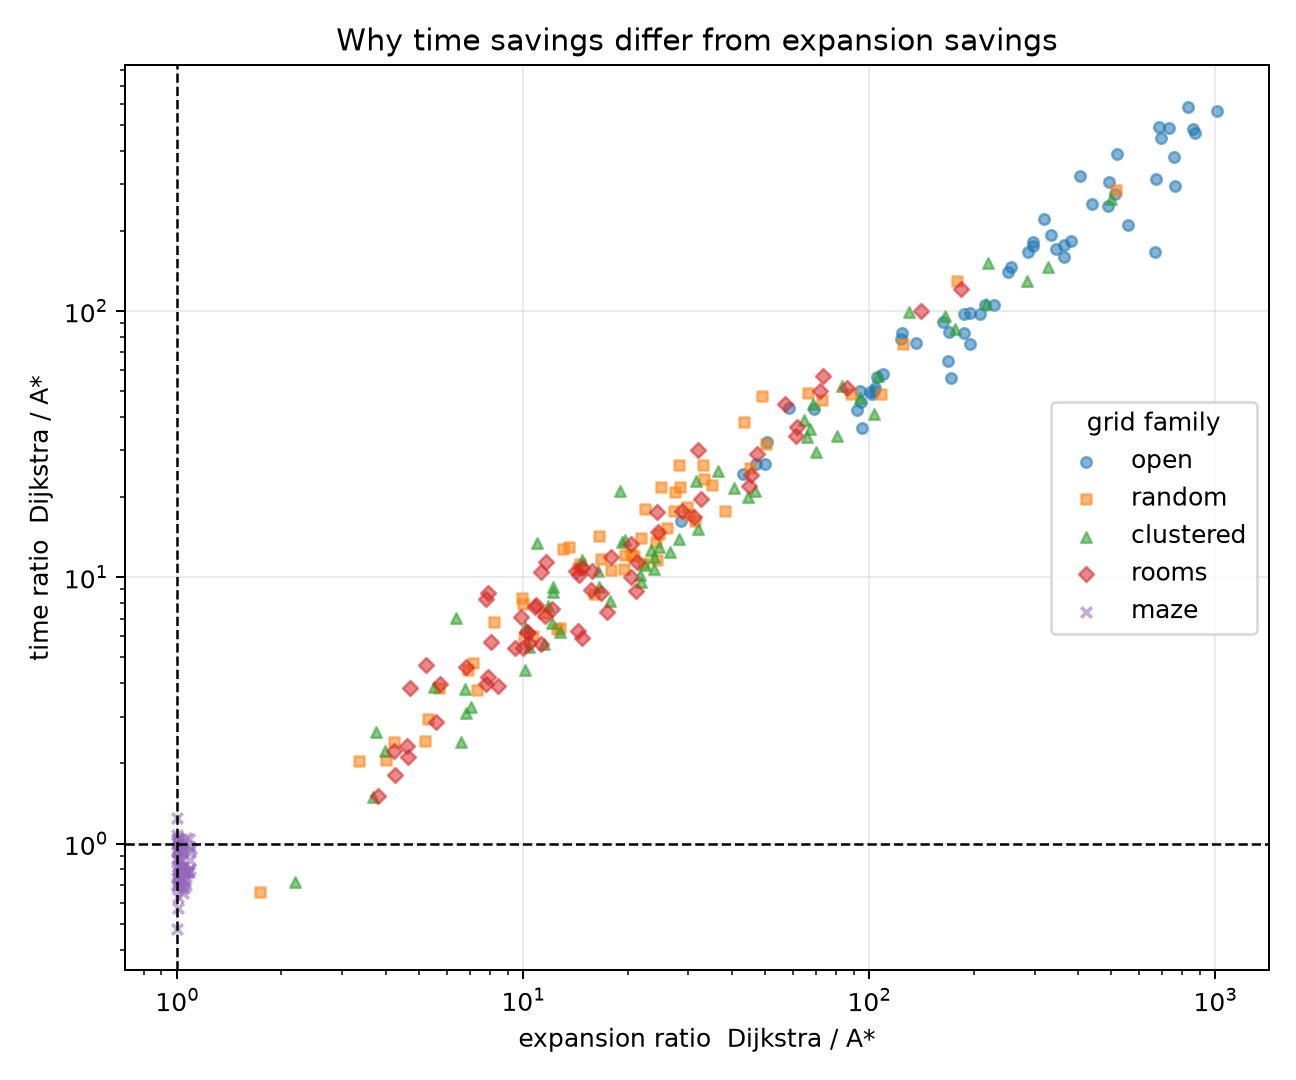
\includegraphics[width=0.80\columnwidth]{../figures/grid_time_vs_expansion.png}
  \caption{Per-query expansion ratio versus time ratio.  Points below the
  diagonal have time savings smaller than expansion savings; this is the
  expected effect of the per-expansion overhead.}
  \label{fig:scatter}
\end{figure}

\subsection{Tie-breaking}
The \code{larger\_g} rule has a median expansion ratio of 1.00 on the open grid
relative to \code{node\_id}, but \code{node\_id} is worse on 45\% of open-grid
queries, up to 285.7x.  The corresponding fractions are 63\% (random), 68\%
(clustered), 58\% (rooms) and 2\% (maze).  On open and clustered grids
\code{larger\_g} never expanded more vertices; on random grids the worst
regression was 0.8\%.  Tie-breaking is therefore a tail-risk decision rather than
a universal median effect.  It never changes the returned distance.

The frozen run also contains both tie-break rules on the real road graph with
ALT K=8.  There, \code{node\_id} expands a median 1.14x as many vertices
(+13.8\%), is worse on 27 of 30 queries, and reaches 2.39x on the worst query
(paired Wilcoxon $p=4.4\times10^{-6}$).  Median wall-clock time is 1.09x, but
that difference is noisy ($p=0.124$).  The expansion count is the reliable
signal, and it confirms the grid conclusion: \code{larger\_g} is a justified
default rather than a cosmetic choice.

A final mechanism check counts maximal equal-\(f\) plateaus, where the
tie-break can change the order: the open grid is one saturated plateau
(median longest run \(=1.00\)), the maze has almost none (\(0.002\)), and the
road graph is intermediate (\(0.35\)).  On the road graph, longer plateaus
predict a larger \code{node\_id} penalty (expansion \(\rho=0.53\), \(p=0.003\)).

\begin{table}[!t]
\centering
\caption{Road graph: queries grouped by the longest equal-\(f\) plateau
(low/mid/high tertiles).  Ratios are node\_id / larger\_g.}
\label{tab:plateau}
\footnotesize
\setlength{\tabcolsep}{4pt}
\begin{tabular}{lcccc}
\toprule
tertile & plateau share & exp ratio & time ratio & worst time\\
\midrule
low  & 0.128 & 1.055 & 1.017 & 1.278\\
mid  & 0.349 & 1.155 & 1.070 & 2.402\\
high & 0.715 & 1.337 & 1.247 & 2.181\\
\bottomrule
\end{tabular}
\end{table}

\begin{figure*}[!t]
  \centering
  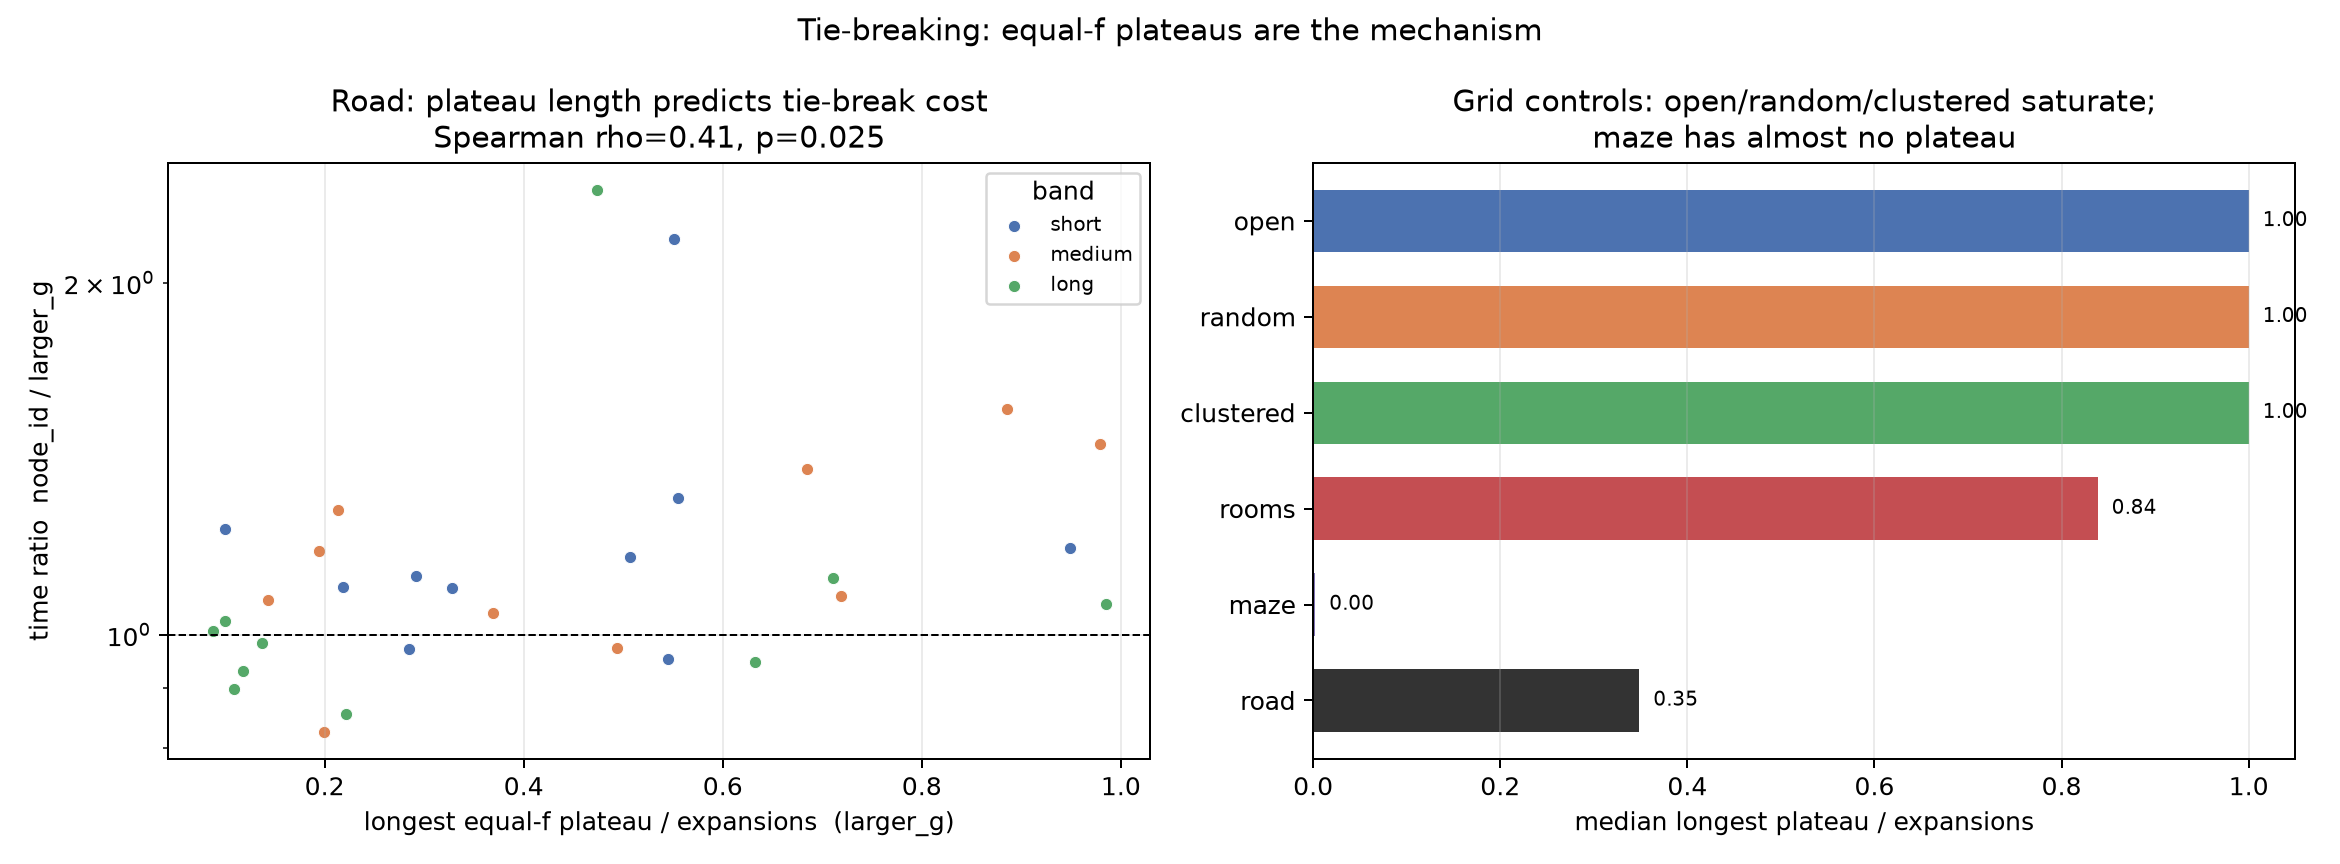
\includegraphics[width=0.88\textwidth]{../figures/tie_plateau.png}
  \caption{Equal-\(f\) plateaus explain tie-break sensitivity.  Left: road
  queries; longer plateaus predict a larger \code{node\_id} cost.  Right:
  median longest plateau by workload.  Open/random/clustered grids are
  saturated; the maze has almost no plateau.}
  \label{fig:plateau}
\end{figure*}


\subsection{Heuristic informativeness}
\label{sec:informativeness}

The expansion result is descriptive; we now ask what makes a heuristic useful.
For each grid query we run BFS from the target, sample 5,000 vertices, and
compare $h(v)$ with the true distance $d(v,t)$.  We report Spearman correlation,
normalised mean absolute error $\mathrm{MAE}/\overline{d}$, detour ratio
$d(s,t)/\mathrm{Manhattan}(s,t)$, and effective branching factor.

Table~\ref{tab:diagnostics} shows the expected ordering.  The open grid has an
exact heuristic: correlation 1.00, normalised MAE 0.00.  Random, clustered and
room grids retain a high rank correlation (0.99) but have growing error
(0.02--0.06); their speedups fall from 105.7x to 8.7--12.8x.  The maze has
correlation 0.42 and normalised MAE 0.97; its speedup is 0.81x.

Across all 300 grid queries, the pooled Spearman correlation is $+0.78$ for
$h$--distance correlation and $-0.81$ for normalised MAE.  A single-feature
least-squares model $\log(T_D/T_A) \sim \mathrm{MAE}/\overline{d}$ has
$R^2=0.55$.  This is an explanatory model, not a universal predictor: within one
family the error range is narrow, and leave-one-family-out extrapolation to the
maze is poor.  The mechanism is nevertheless clear: admissibility is not
enough; the heuristic must be \emph{informative} about the actual remaining
distance.

On the road graph (ALT K=8), the heuristic is also informative:
$h$--distance correlation 0.98, normalised MAE 0.155.  The query-level Spearman
correlation between absolute heuristic error and time ratio is $-0.77$.

\begin{table}[!t]
\centering
\caption{Heuristic diagnostics and outcomes (grid medians; exploratory).}
\label{tab:diagnostics}
\footnotesize
\setlength{\tabcolsep}{2.5pt}
\begin{tabular}{lccccc}
\toprule
Family & $h$ corr. & norm. MAE & detour & time ratio & EBF A*\\
\midrule
Open & 1.00 & 0.00 & 1.00 & 105.7x & 1.00\\
Random & 1.00 & 0.02 & 1.00 & 12.8x & 1.02\\
Clustered & 0.99 & 0.04 & 1.00 & 12.8x & 1.01\\
Rooms & 0.99 & 0.06 & 1.02 & 8.7x & 1.02\\
Maze & 0.42 & 0.97 & 35.06 & 0.81x & 1.00\\
\bottomrule
\end{tabular}
\end{table}

\begin{figure*}[!t]
  \centering
  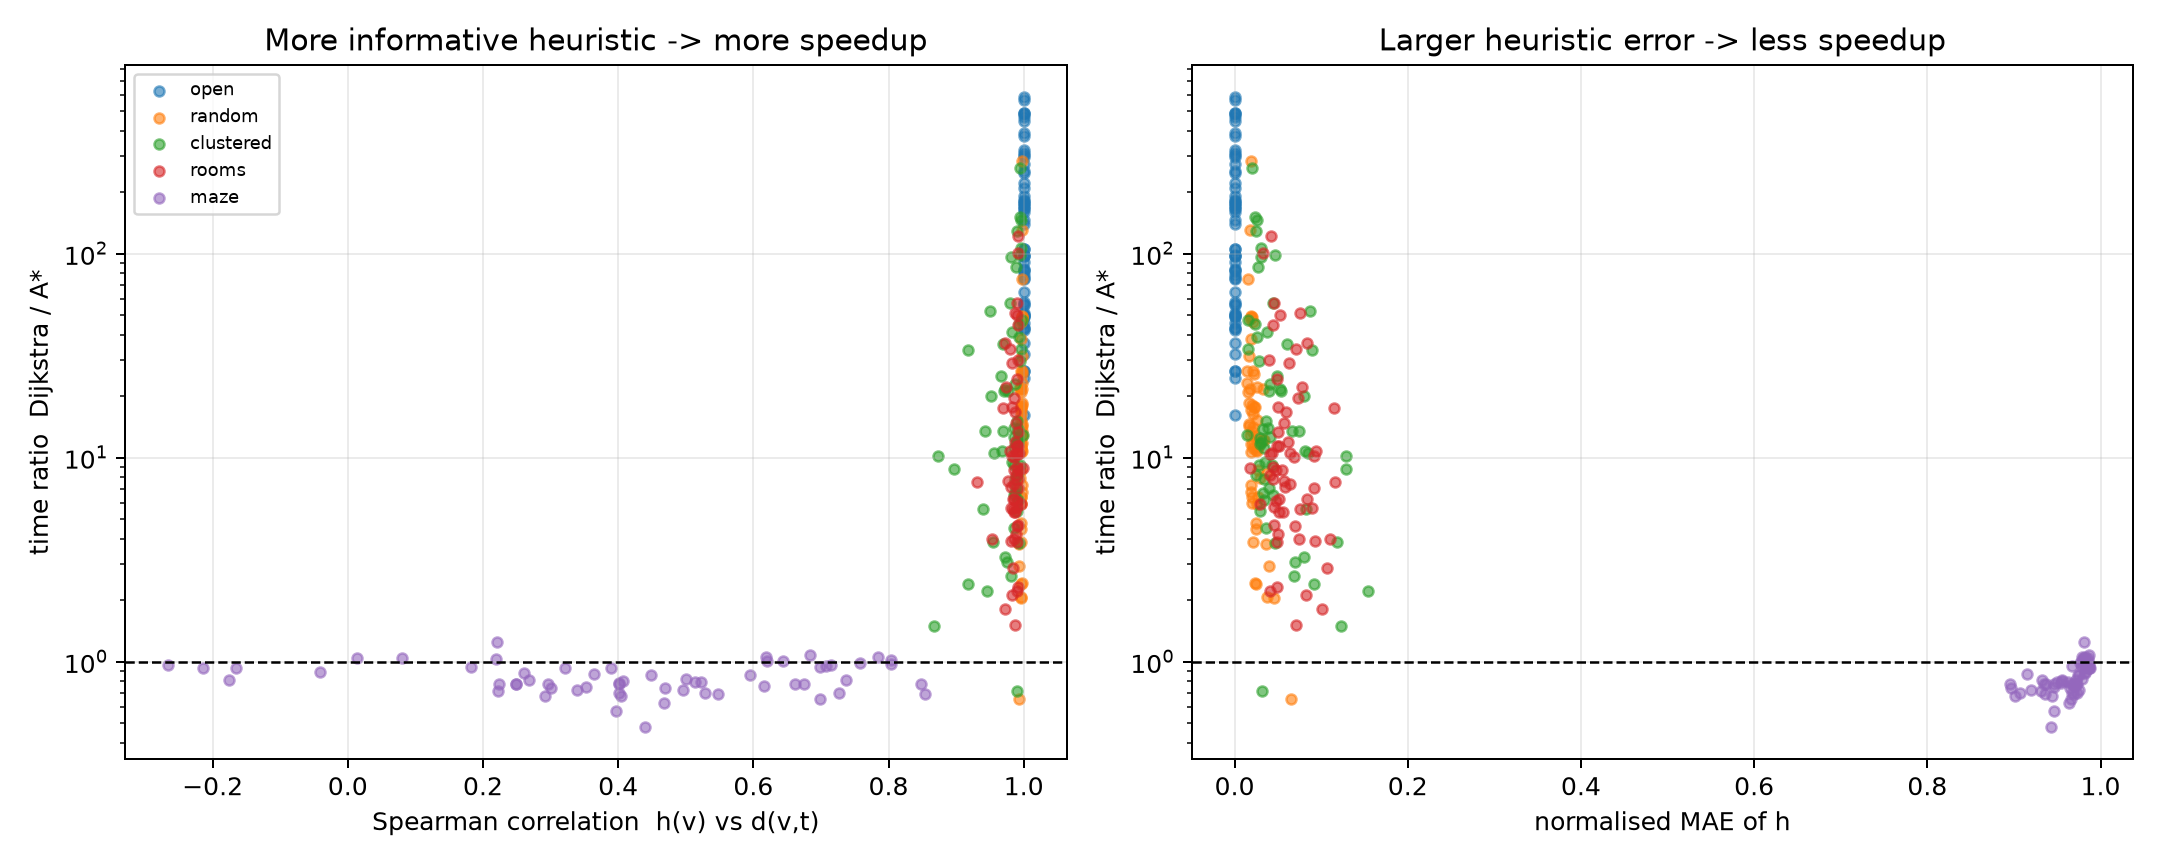
\includegraphics[width=0.72\textwidth]{../figures/novelty_heuristic_speedup.png}
  \caption{Heuristic informativeness versus speedup.  Left: rank correlation
  between $h(v)$ and the true remaining distance.  Right: normalised MAE.
  The maze is the low-information, low-speedup outlier.}
  \label{fig:info}
\end{figure*}

\subsection{Price of optimality: weighted \Astar{}}
\label{sec:weighted}

The maze is the negative case for optimal \Astar{}.  We therefore test the
weighted objective $f=g+\epsilon h$ on all five grid families and the road
graph, with
$\epsilon\in\{1,1.1,1.25,1.5,2,3,5,10,20,50\}$.  The primary results use a
closed list, where a settled vertex is not reopened; reopening is retained as a
sensitivity check because it is the aggressive choice.  All weighted runs
returned at least the optimal distance; $\epsilon=1$ was exact under both
policies.  Table~\ref{tab:weighted} shows selected rows.

A perfect maze has a unique simple path between two cells, so every returned
path has the same cost.  The measured path-cost ratio is exactly 1.00 for every
$\epsilon$, and at $\epsilon=50$ weighted \Astar{} is 1.10x faster than
Dijkstra.  The optimality price is therefore zero on this control, but only
because there is nothing to trade.

On graphs with alternative paths the trade is real and depends on the base
heuristic.  With the closed list, random obstacles at $\epsilon=1.1$ improve
the median speedup from 12.8x to 20.1x for a 1.8\% median cost increase;
$\epsilon=1.25$ reaches 38.2x for 5.5\%.  Rooms at $\epsilon=1.25$ reach 24.8x
for 3.1\%, and clustered obstacles at $\epsilon=1.5$ reach 26.5x for 5.0\%.
The open grid is the control where Manhattan is exact: cost stays 1.00 and
weighting cannot reduce expansions further.

The road graph exposes the policy choice.  Optimal ALT K=8 is 7.4x faster than
Dijkstra in this sweep; the closed-list $\epsilon=1.1$ variant reaches 8.8x at
1.4\% median cost, while reopening the same $\epsilon$ collapses to 5.4x.  Where the
heuristic is already tight, reheapifying settled vertices costs more than the
shorter search saves.  Weighting is thus useful when the heuristic is weak, not
as a universal speed switch, and the closed list is the better default for this
implementation.

\begin{table*}[!t]
\centering
\caption{Weighted \Astar{} with a closed list (except the last row).  Ratio is
Dijkstra/weighted \Astar{}; cost is returned path cost divided by the optimal
cost.  Selected $\epsilon$ values; the full sweep has ten values.}
\label{tab:weighted}
\footnotesize
\setlength{\tabcolsep}{6pt}
\begin{tabular}{llcccccc}
\toprule
workload & policy & $\epsilon$ & time ratio & cost median & cost p95 & cost max\\
\midrule
random      & closed & 1.10 & 20.1x & 1.018 & 1.06 & 1.07\\
random      & closed & 1.25 & 38.2x & 1.055 & 1.13 & 1.15\\
rooms       & closed & 1.25 & 24.8x & 1.031 & 1.09 & 1.11\\
clustered   & closed & 1.50 & 26.5x & 1.050 & 1.15 & 1.21\\
road        & closed & 1.00 & 7.4x  & 1.000 & 1.00 & 1.00\\
road        & closed & 1.10 & 8.8x  & 1.014 & 1.04 & 1.04\\
road        & reopen & 1.10 & 5.4x  & 1.011 & 1.04 & 1.04\\
\bottomrule
\end{tabular}
\end{table*}

\begin{figure*}[!t]
  \centering
  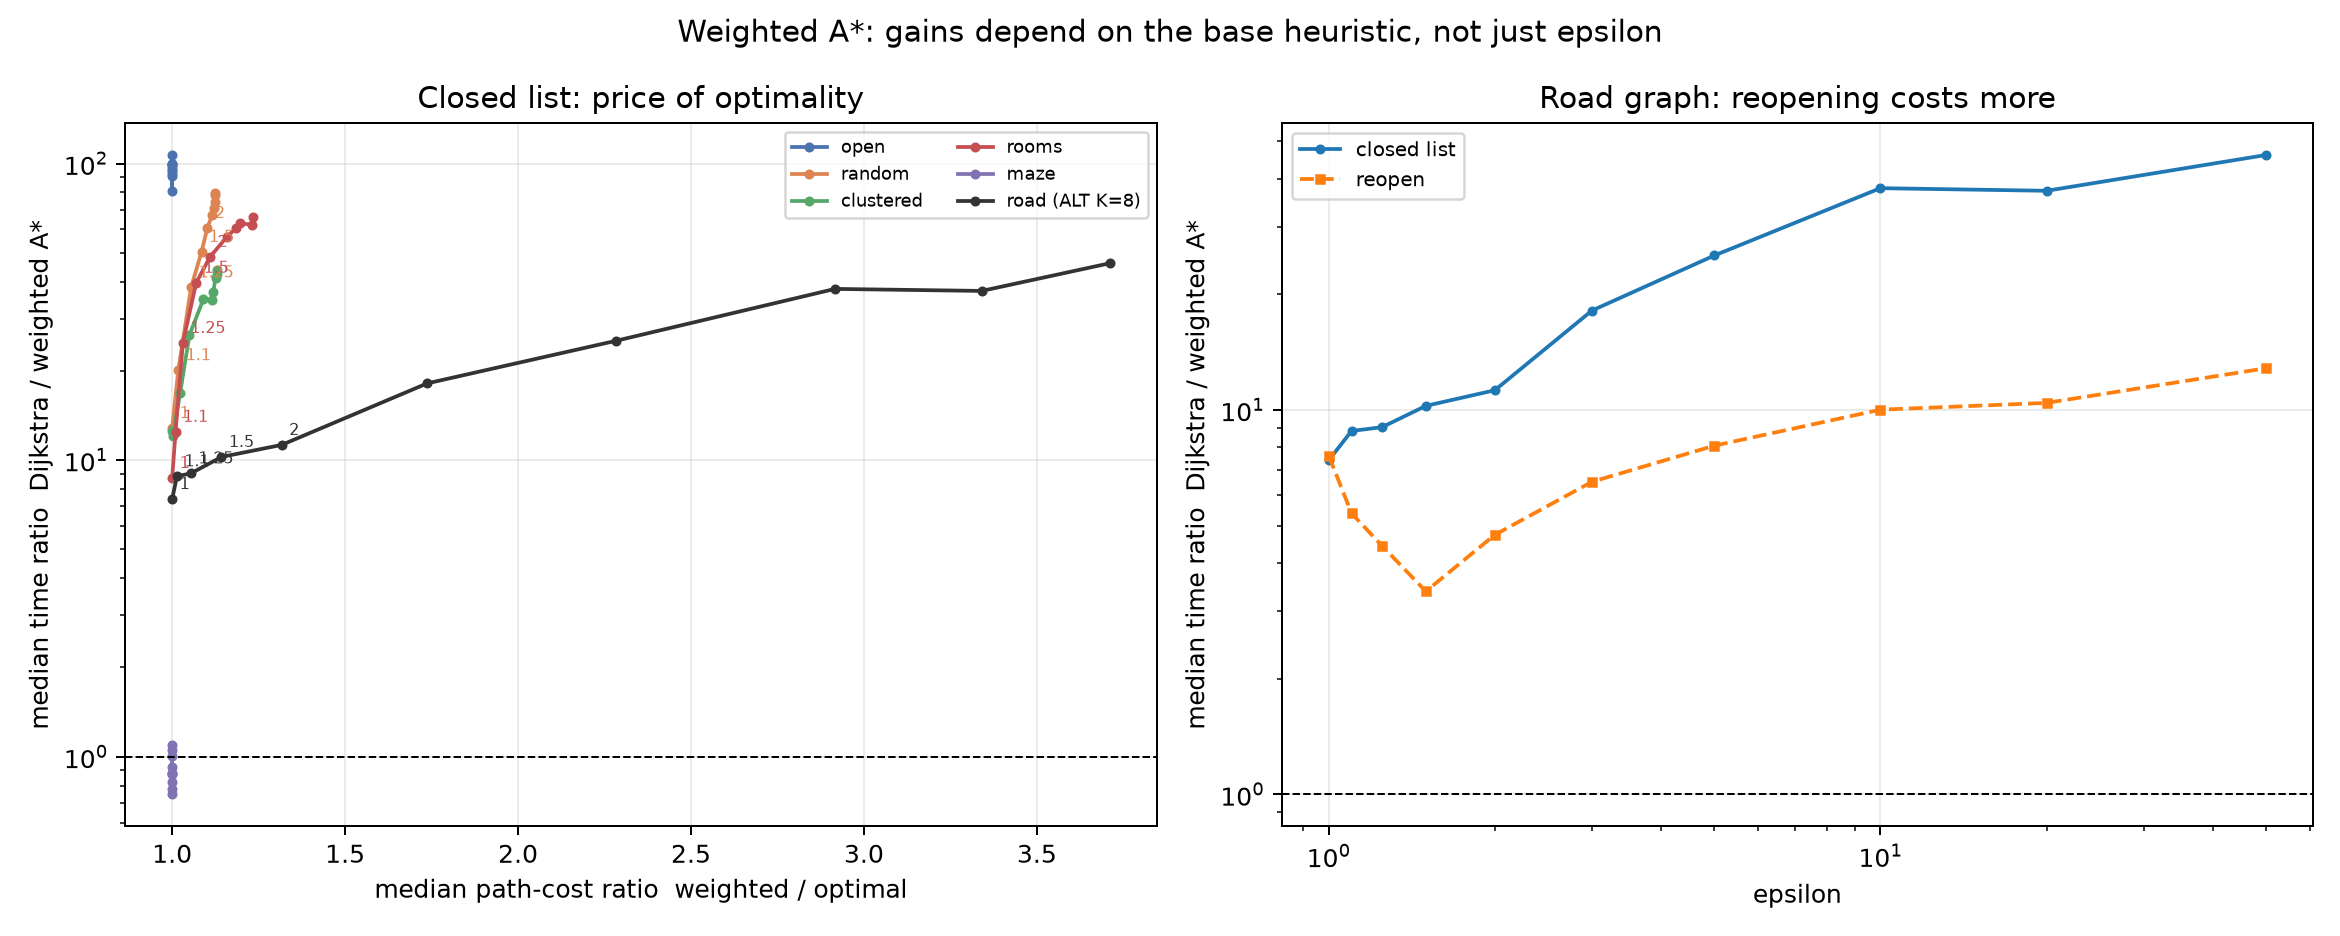
\includegraphics[width=0.72\textwidth]{../figures/weighted_pareto.png}
  \caption{Weighted \Astar{} on graphs with alternative paths.  Left:
  closed-list cost versus speed, with selected $\epsilon$ labels.  Right: on
  the road graph the closed list is faster at every $\epsilon>1$, while
  reopening churns the heap for no useful gain.  The open grid and perfect maze
  sit at cost ratio 1.00 because they leave no alternative path to trade.}
  \label{fig:weighted}
\end{figure*}



\subsection{Weighted road network}
\label{sec:weighted-road}

The frozen road graph is unit-hop.  As a separate data regime we use the DIMACS
\code{USA-road-d.NY} graph \cite{dimacs}: 264,346 nodes, 730,100 undirected
weighted arcs after symmetrisation, integer distance weights, and coordinates.
Weighted Dijkstra supplies the oracle, the ALT tables are built with weighted
Dijkstra, and queries are selected in weighted-distance bands.  All 30 queries
return the weighted optimum for every treatment.

\begin{table}[!t]
\centering
\caption{Weighted New York road graph: median time and expansion ratios
(Dijkstra / A*).  All 30 queries return the weighted optimum.}
\label{tab:weighted-road}
\footnotesize
\setlength{\tabcolsep}{4pt}
\begin{tabular}{lcc}
\toprule
treatment & time ratio & expansion ratio\\
\midrule
Euclidean A* & 1.6x & 1.9x\\
ALT K=1 & 1.6x & 2.3x\\
ALT K=4 & 10.0x & 14.6x\\
ALT K=8 & \textbf{18.4x} & \textbf{25.8x}\\
ALT K=16 & \textbf{21.6x} & \textbf{31.1x}\\
\bottomrule
\end{tabular}
\end{table}

Euclidean A* is admissible but weak: the straight-line bound is much looser
than landmark distances, so it gives only 1.6x.  ALT K=16 is the fastest
treatment; K=8 is close.  This ranking is the same as in the unit-hop
California graph, but the absolute speedups are not directly comparable because
the graph and query set differ.

\begin{figure*}[!t]
  \centering
  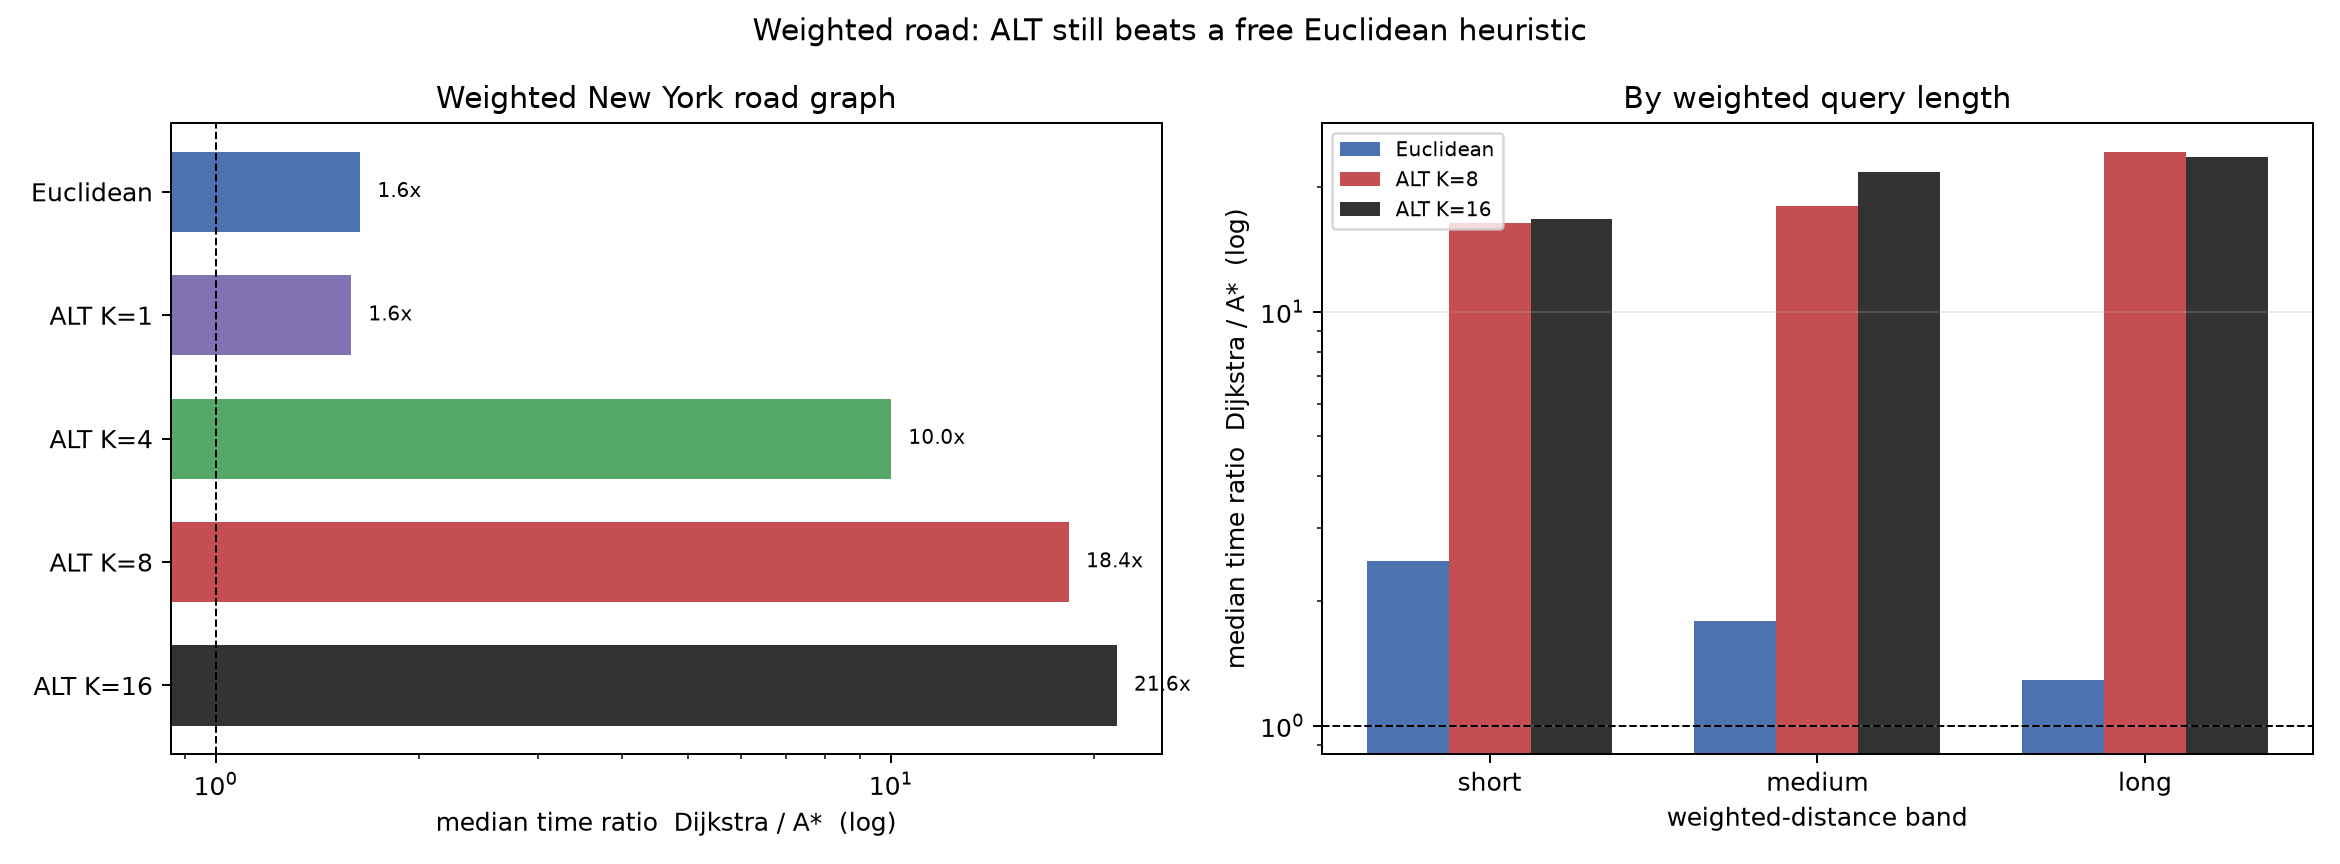
\includegraphics[width=0.88\textwidth]{../figures/weighted_road.png}
  \caption{Weighted New York road graph.  Left: median time ratio for
  Euclidean A* and ALT.  Right: speedup by weighted-distance band.  ALT's
  advantage grows with landmarks; the free Euclidean bound is weak on long
  queries.}
  \label{fig:weighted-road}
\end{figure*}

\subsubsection{Weighted A* on the weighted graph}
The same weighted graph also supports the price-of-optimality experiment.  We
sweep \(f=g+\epsilon h\) with ALT K=8, both closed-list and reopening policies,
and use the weighted distance as the path cost.  Table~\ref{tab:weighted-road-eps}
reports the full sweep.  The first percent is cheap: the closed-list
\(\epsilon=1.1\) variant reaches 35.1x for a 1.1\% median cost increase, and
\(\epsilon=1.25\) reaches 53.9x for 4.1\%.  Reopening is slower at every
\(\epsilon>1\), and the speedup saturates above \(\epsilon\approx3\) while the
cost continues to rise.

\begin{table*}[!t]
\centering
\caption{Weighted A* on the weighted New York graph (ALT K=8).  Time ratio is
Dijkstra / weighted A*; cost is returned weighted distance / optimum.}
\label{tab:weighted-road-eps}
\footnotesize
\setlength{\tabcolsep}{8pt}
\begin{tabular}{lcccc}
\toprule
& \multicolumn{2}{c}{closed list} & \multicolumn{2}{c}{reopen}\\
\cmidrule(lr){2-3}\cmidrule(lr){4-5}
\(\epsilon\) & time ratio & cost ratio & time ratio & cost ratio\\
\midrule
1.00 & 16.0x & 1.000 & 16.1x & 1.000\\
1.10 & 35.1x & 1.011 & 27.0x & 1.013\\
1.25 & 53.9x & 1.041 & 35.1x & 1.039\\
1.50 & 77.1x & 1.060 & 51.0x & 1.061\\
2.00 & 99.8x & 1.092 & 80.8x & 1.089\\
3.00 & 102.2x & 1.146 & 87.0x & 1.137\\
5.00 & 115.9x & 1.167 & 91.5x & 1.156\\
10.0 & 121.7x & 1.213 & 103.0x & 1.207\\
20.0 & 121.4x & 1.255 & 103.7x & 1.237\\
50.0 & 123.9x & 1.247 & 110.5x & 1.234\\
\bottomrule
\end{tabular}
\end{table*}

\begin{figure*}[!t]
  \centering
  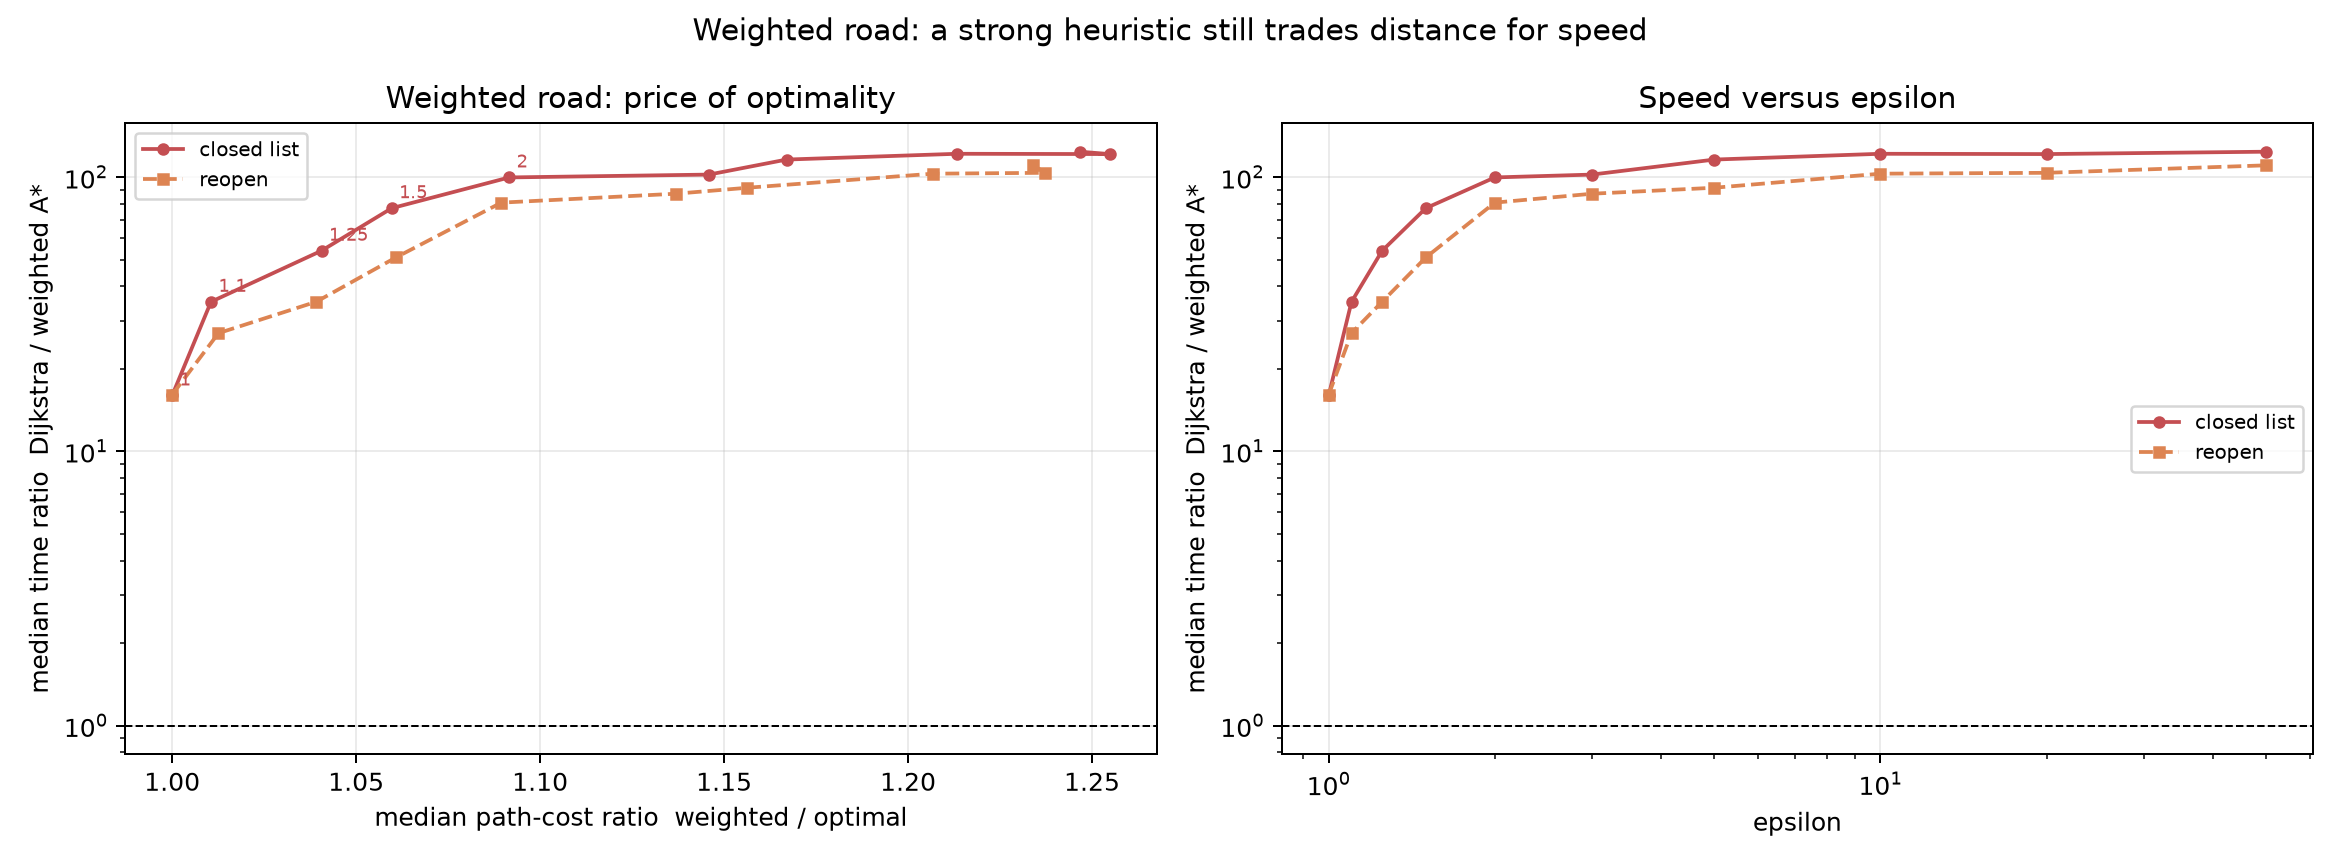
\includegraphics[width=0.86\textwidth]{../figures/weighted_road_eps.png}
  \caption{Weighted A* on the weighted road graph.  Left: cost-speed frontier;
  labels are \(\epsilon\).  Right: speed versus \(\epsilon\) for closed-list
  and reopening policies.  The closed list is faster for essentially the same
  path cost.}
  \label{fig:weighted-road-eps}
\end{figure*}

\subsubsection{Same-topology unit-weight control}
To isolate the effect of weights, we rerun the \emph{identical} 30
source-target pairs on the same topology with every edge weight set to 1.  The
unit run recomputes BFS ALT landmarks and uses a BFS hop-distance oracle.  The
weighted and unit runs therefore differ only in the edge weights and the
corresponding oracle/heuristic tables.

\begin{table}[!t]
\centering
\caption{Same topology and query pairs: distance weights versus unit weights.
Time ratio is Dijkstra / A*.}
\label{tab:unit-road}
\footnotesize
\setlength{\tabcolsep}{4pt}
\begin{tabular}{lcccc}
\toprule
& \multicolumn{2}{c}{time ratio} & \multicolumn{2}{c}{expansion ratio}\\
\cmidrule(lr){2-3}\cmidrule(lr){4-5}
treatment & weighted & unit & weighted & unit\\
\midrule
ALT K=1 & 1.59 & 1.41 & 2.25 & 2.16\\
ALT K=4 & 10.02 & 7.84 & 14.57 & 13.15\\
ALT K=8 & \textbf{18.37} & \textbf{10.36} & \textbf{25.76} & \textbf{17.70}\\
ALT K=16 & \textbf{21.62} & \textbf{13.56} & \textbf{31.09} & \textbf{23.90}\\
ALT K=8, node\_id & 15.22 & 9.63 & 18.73 & 14.74\\
\bottomrule
\end{tabular}
\end{table}

Distance weights make ALT substantially more valuable: ALT K=8 improves from
10.4x on unit weights to 18.4x on distance weights, a 1.77x increase in the
speedup.  They also reduce tie sensitivity: the median \code{node\_id} /
\code{larger\_g} time penalty falls from 1.17x to 1.08x, and the expansion
penalty from 1.19x to 1.08x.  The ranking is unchanged; weights change the size
of the advantage, not which algorithm wins.

\begin{figure*}[!t]
  \centering
  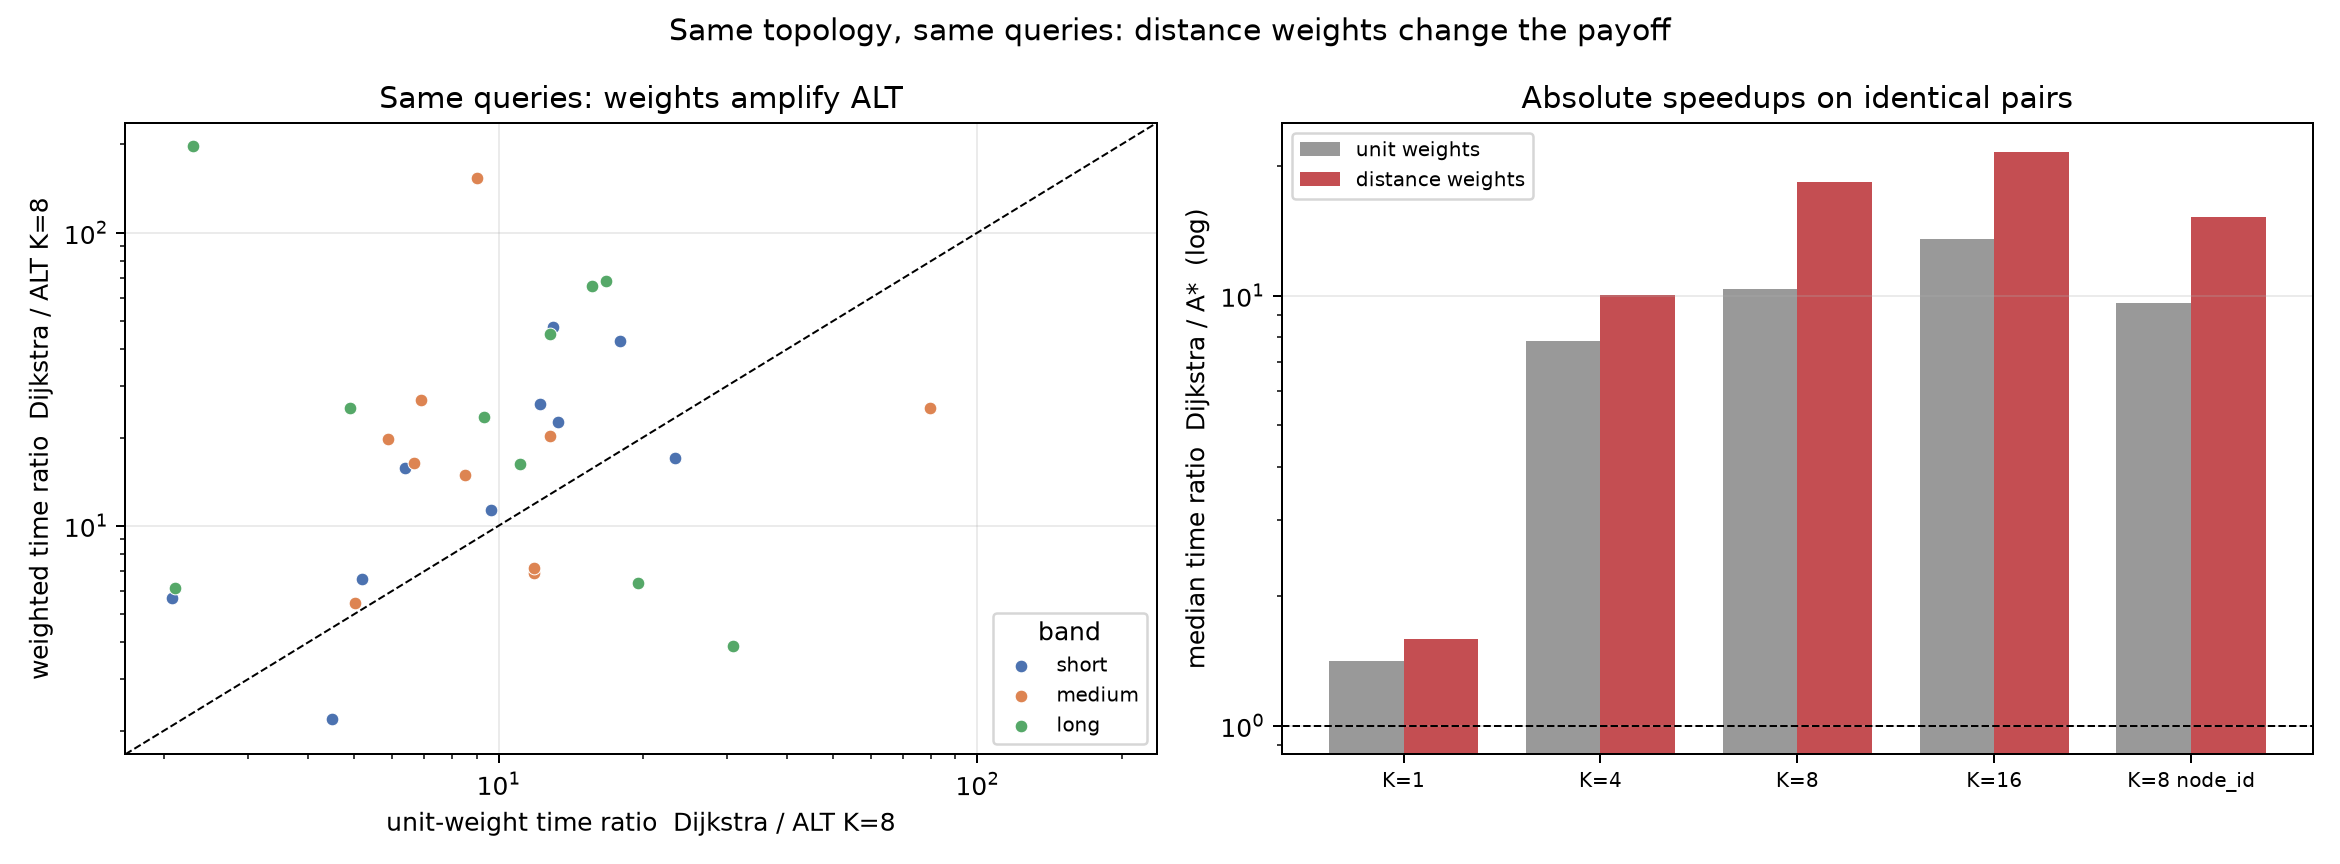
\includegraphics[width=0.88\textwidth]{../figures/unit_road.png}
  \caption{Same topology, same source-target pairs: distance weights versus
  unit weights.  Left: per-query ALT K=8 speedups; points above the diagonal
  improve under weights.  Right: absolute speedups by treatment.}
  \label{fig:unit-road}
\end{figure*}

\subsection{Batch throughput with OpenMP}
\label{sec:omp}

The problem statement asks about one query at a time, and a single A*/Dijkstra
search is inherently sequential.  Independent queries, however, are
embarrassingly parallel.  We run the five $1024^2$ grid families and the 30 road
queries (three repeats each) with 1, 2, 4, 8 and 16 OpenMP threads.  Each task
still runs Dijkstra and A* sequentially on the same query; each worker gets its
own search scratch and heuristic object.  Input construction, query selection
and thread-local scratch allocation are outside the timed parallel region.
The frozen query-level results remain serial.

Table~\ref{tab:omp} shows 9.73x batch throughput at 16 threads (61\% parallel
efficiency): 9.93x for the grid workload and 9.36x for the road workload.  The
sublinear scaling is expected from the mix of performance and efficiency cores
and from memory bandwidth.  The efficiencies slightly above one at two and four
threads are within frequency/run-to-run variation, not super-linear scaling.  Per-query latency inflates by 21\% for Dijkstra and
18\% for A* at 16 threads; the median Dijkstra/A* ratio rises from 14.8x to
17.9x, and the maze remains below parity (0.87x).  The structural conclusion is
therefore unchanged under parallel load.  This is a throughput result, not a
claim that a single query becomes faster.

\begin{table}[!t]
\centering
\caption{OpenMP batch throughput (five $1024^2$ grids plus the road graph).}
\label{tab:omp}
\footnotesize
\setlength{\tabcolsep}{3pt}
\begin{tabular}{rccc}
\toprule
Threads & Batch time & Speedup & Efficiency\\
\midrule
1 & 44.39 s & 1.00x & 1.00\\
2 & 21.48 s & 2.07x & 1.03\\
4 & 10.11 s & 4.39x & 1.10\\
8 & 6.27 s & 7.08x & 0.89\\
16 & 4.56 s & 9.73x & 0.61\\
\bottomrule
\end{tabular}
\end{table}

\section{Discussion}
\label{sec:discussion}

Table~\ref{tab:hyp} summarizes the pre-registered predictions.  H1--H4 were
confirmed.  H5 was only partly confirmed: open-grid long queries benefit more
than short ones, but random-grid long queries do not.  H6 was partly rejected:
K=8 is strong, K=1 does not produce a significant time saving, but K=16 is
still better than K=8 rather than a plateau.  H7 was rejected as a median
claim; the tie-break matters in a heavy tail.

\begin{table}[!t]
\centering
\caption{Hypothesis outcomes.}
\label{tab:hyp}
\footnotesize
\setlength{\tabcolsep}{3pt}
\begin{tabular}{p{0.6cm}p{5.5cm}p{1.5cm}}
\toprule
 & Prediction & Outcome\\
\midrule
H1 & Open: \Astar{} saves many expansions and time & confirmed\\
H2 & Random: saves, less than open & confirmed\\
H3 & Clustered/rooms weaker; rooms weaker than random & confirmed\\
H4 & Maze: no expansion saving; \Astar{} slower & confirmed\\
H5 & Long queries benefit more than short & partly rejected\\
H6 & ALT K=8 strong; K=1 weak; plateau at 16 & partly rejected\\
H7 & \code{larger\_g} reduces median expansions on open & rejected\\
\bottomrule
\end{tabular}
\end{table}

The exploratory diagnostics explain the table: the practical rule is not
``\Astar{} is faster than Dijkstra.''  It is: \emph{\Astar{} is faster when
the heuristic is informative enough that the expansion reduction exceeds the
per-expansion overhead.}  Weighted \Astar{} can buy speed when the heuristic
is weak but admissible: on random obstacles it reaches 20.1x for 1.8\% median
cost, while the perfect maze remains a zero-price control because its path is
unique.  On the road graph the heuristic is already tight, so reopening costs
more than it saves and the closed-list gain is modest (7.4x to 8.8x at 1.4\%
cost).  The OpenMP batch result shows a separate, engineering
gain: independent queries scale to 9.73x throughput at 16 threads without
changing which algorithm wins per query.  Open grids satisfy
this overwhelmingly; random, clustered and room grids satisfy it comfortably;
the road graph satisfies it with ALT; the maze does not.

The result also explains why a strong but expensive heuristic can still win on
the road graph.  K=16 evaluates 16 landmark differences per generated vertex,
but the expansion count falls enough that the net time is lower than K=8.

\section{Threats to Validity}
\label{sec:threats}

The main external-validity threat is the single real graph.  \code{roadNet-CA}
is a sparse, near-planar road network; the result should not be generalized to
dense social graphs, directed one-way networks or weighted travel-time routing
without repeating the experiment.  SNAP supplies no road lengths or travel
times, so the real graph is unit-cost.  The grids are synthetic controls; they
isolate structure but are not a sample of real maps.  We symmetrise roads, so
one-way streets are not modelled.

The timing is single-machine wall-clock time.  The reported run was collected
with the host in its lowest performance/power mode.  Absolute nanoseconds are
therefore mode-specific; the paired ratios are the primary result.  We reran a
matched subset in the host's higher performance mode: 150 grid queries at sizes
128 and 512 plus all 30 road queries, with the frozen seeds, bands and repeats.
Both algorithms became about 2.24x faster, while the Dijkstra/\Astar{} ratio
changed by only 1.011 on grids (95\% CI 0.994--1.028, $p=0.90$) and 0.993 on the
road graph (0.967--1.020, $p=0.21$); expansion counts were identical.  We reduce
noise by pinning one CPU, using one warm-up, repeating runs and reporting
medians, IQRs, bootstrap intervals and paired tests.  The median within-query CV
is 7--10\%, much smaller than the reported treatment ratios, except for the
explicitly non-significant K=1 road result.  A different heap or compiler
could change constants, but not the mechanism.

The open-grid result is partly a tie-breaking effect.  With \code{node\_id},
open-grid \Astar{} still expands 54x fewer vertices than Dijkstra, but
\code{larger\_g} raises that to 222x.  The main treatment was fixed in the
protocol; the tie-break study is reported separately.

\section{Conclusion}
\label{sec:conclusion}

We compared Dijkstra and \Astar{} under a frozen paired protocol on five grid
families and a real road network.  \Astar{} is worth using when the heuristic
captures the structure of the remaining path: on open grids it is 105.7x faster
with 222.4x fewer expansions, and on a road network with ALT K=8 it is 7.62x
faster with 11.54x fewer expansions (K=16: 13.52x and 22.41x).  It is not worth
using in a perfect maze, where it is 24\% slower because Manhattan distance does
not see the forced turns.  Across all cases, time savings are smaller than
expansion savings because \Astar{} costs 1.2--2.0x more per expansion.  The right question is therefore not whether \Astar{} is better in general, but
whether the heuristic is informative enough for the expansion saving to pay for
the guidance.  A follow-up diagnostic supports this: heuristic error predicts
the speedup, and weighted \Astar{} with a closed list turns a small path-cost
budget into a large gain when the heuristic is weak (random obstacles: 20.1x for
1.8\% median cost).  On the road graph, where the heuristic is already tight,
reopening costs more than it saves; the closed-list variant improves the
optimal ALT speedup from 7.4x to 8.8x at 1.4\% cost.  The real-graph tie-break
check also confirms that \code{larger\_g} is the safer default: the
\code{node\_id} rule expands 1.14x as many vertices and is worse on 27 of 30
queries.
For batch workloads, independent queries add a further 9.73x throughput at 16
threads while preserving the per-query ranking.  Finally, rerunning a matched
subset in the host's higher performance mode made both algorithms about 2.24x
faster but changed the Dijkstra/\Astar{} ratio by only 0.011 on grids and
$-0.007$ on the road graph, so the ranking is not an artefact of the host power
mode.

\section*{Reproducibility}
Source, tests, frozen protocol, raw data, scripts and figures are in the
project repository.  The main run uses seed 20261030, 3 grid repeats and 5 road
repeats, and all 3,600 runs are checked against a BFS oracle.  The full
experiment is reproduced with
\code{./scripts/run\_experiments.sh}; the exploratory analyses with
\code{./scripts/run\_novelty.sh}; and the OpenMP study with
\code{./scripts/run\_omp.sh}.

\begin{thebibliography}{00}
\bibitem{dijkstra1959}
E. W. Dijkstra, ``A note on two problems in connexion with graphs,''
\emph{Numerische Mathematik}, vol. 1, pp. 269--271, 1959.

\bibitem{hart1968}
P. E. Hart, N. J. Nilsson, and B. Raphael, ``A formal basis for the heuristic
determination of minimum cost paths,'' \emph{IEEE Trans. Syst. Sci. Cybern.},
vol. 4, no. 2, pp. 100--107, 1968.

\bibitem{goldberg2005}
A. V. Goldberg and C. Harrelson, ``Computing the shortest path: \Astar{} search
meets graph theory,'' in \emph{Proc. ACM--SIAM Symp. Discrete Algorithms
(SODA)}, 2005, pp. 156--165.

\bibitem{russell2020}
S. Russell and P. Norvig, \emph{Artificial Intelligence: A Modern Approach},
4th ed. Hoboken, NJ, USA: Pearson, 2020.

\bibitem{snap}
J. Leskovec and A. Krevl, ``SNAP Datasets: Stanford large network dataset
collection,'' 2014. [Online]. Available:
\url{https://snap.stanford.edu/data/roadNet-CA.html}

\bibitem{dimacs}
C. Demetrescu, A. V. Goldberg, and D. S. Johnson, Eds., \emph{The Shortest Path
Problem: Ninth DIMACS Implementation Challenge}. DIMACS Series in Discrete
Mathematics and Theoretical Computer Science, 2009.

\bibitem{cormen2022}
T. H. Cormen, C. E. Leiserson, R. L. Rivest, and C. Stein, \emph{Introduction
to Algorithms}, 4th ed. Cambridge, MA, USA: MIT Press, 2022.
\end{thebibliography}

\end{document}
